\documentclass[a4paper,12pt]{article}

%%% Работа с русским языком
\usepackage{cmap}					% поиск в PDF
\usepackage{mathtext} 				% русские буквы в формулах
\usepackage[T2A]{fontenc}			% кодировка
\usepackage[utf8]{inputenc}			% кодировка исходного текста
\usepackage[english,russian]{babel}	% локализация и переносы
\usepackage{xcolor}
\usepackage{hyperref}
 % Цвета для гиперссылок
\definecolor{linkcolor}{HTML}{799B03} % цвет ссылок
\definecolor{urlcolor}{HTML}{799B03} % цвет гиперссылок

\hypersetup{pdfstartview=FitH,  linkcolor=linkcolor,urlcolor=urlcolor, colorlinks=true}

%%% Дополнительная работа с математикой
\usepackage{amsfonts,amssymb,amsthm,mathtools} % AMS
\usepackage{amsmath}
\usepackage{icomma} % "Умная" запятая: $0,2$ --- число, $0, 2$ --- перечисление

%% Номера формул
%\mathtoolsset{showonlyrefs=true} % Показывать номера только у тех формул, на которые есть \eqref{} в тексте.

%% Шрифты
\usepackage{euscript}	 % Шрифт Евклид
\usepackage{mathrsfs} % Красивый матшрифт

%% Свои команды
\DeclareMathOperator{\sgn}{\mathop{sgn}}

%% Перенос знаков в формулах (по Львовскому)
\newcommand*{\hm}[1]{#1\nobreak\discretionary{}
{\hbox{$\mathsurround=0pt #1$}}{}}
% графика
\usepackage{graphicx}
\graphicspath{{pictures/}}
\DeclareGraphicsExtensions{.pdf,.png,.jpg}
\author{Бурмашев Григорий, БПМИ-208}
\title{ТВиМС, дз -- 2}
\date{\today}
\begin{document}
\maketitle
\section*{Задача 7}
\begin{center}

\includegraphics[scale=0.3]{2.png}
\end{center}
\begin{center}
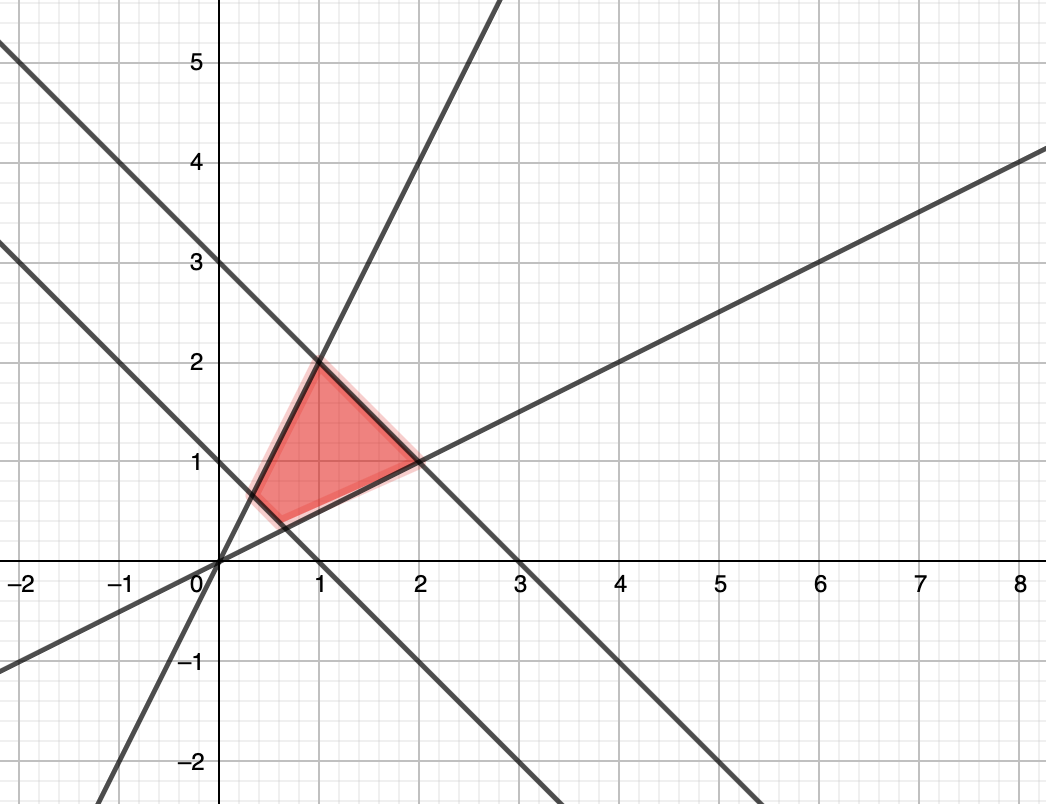
\includegraphics[scale=0.3]{1.png}
\end{center}
\subsection*{a) $q < 1$}
Расписываем достаточное условие для нашего случая, т.к величины положительные произведение тоже положительное и модуль можем убрать (хотим стремление к нулю):
\[
\sum_{n=1}^{\infty} P 
\left(
\prod_{i = 1}^{n} X_i 
\geq \delta 
\right) 
< \infty 
\]
Теперь по указанию от Зеленова вспоминаем про неравенство Чебышева:
\[
P
\left(
\prod_{i= 1}^{n} X_i
\geq \delta
\right) 
\leq
\frac{\prod\limits_{i = 1}^{n} \mathbb{E} X_i }{\delta}
\]
Теперь подгоняем под наш случай, докидываем сумму и избавляемся от произведения справа (из независимости величин получаем просто $q^n$:
\[
\sum_{n=1}^{\infty} P 
\left(
\prod_{i = 1}^{n} X_i
\geq \delta
\right) 
\leq
\sum_{n=1}^{\infty}
\frac{q^n}{\delta}
\]
Теперь для достаточного условия можем зажать через $q^n$, т.е нужно проверить просто:
\[
\sum_{n=1}^{\infty}
\frac{q^n}{\delta} 
< \infty 
\]
Ну а это уже верно, т.к $q < 1$ и такой ряд сходится. Отсюда получаем, что выполняется достаточное условие сходимости п.н  и мы получаем:
\[
\prod_{n = 1}^{N} X_n   \overset{\text{п.н}}{\longrightarrow} 0
\]
\begin{center}
\textbf{Ч.Т.Д} 
\end{center}
\subsection*{b) $q = 1$}
Пользуемся указанием Зеленова и смотрим на $\sqrt{X_n}$ и $\mathbb{E} \sqrt{X_n}$. Заметим (по свойству мат ожидания):
\[
\mathbb{E} X_n > \left(\mathbb{E} \sqrt{X_n}\right)^2 \rightarrow \sqrt{\mathbb{E}X_N} >  \mathbb{E}\sqrt{X_n} \rightarrow 1 > \mathbb{E} \sqrt{X_n}
\]
Теперь можем вновь вернуться к неравенству Чебышева, но уже для корня:
\[
P
\left(
\prod_{i= 1}^{n} \sqrt{X_i}
\geq \delta
\right) 
\leq
\frac{\prod\limits_{i = 1}^{n} \mathbb{E} \sqrt{X_i}}{\delta}
\]
Отсюда:
\[
\sum_{n=1}^{\infty} P 
\left(
\prod_{i = 1}^{n} \sqrt{X_i}
\geq \delta
\right) 
\leq
\sum_{n=1}^{\infty}
\frac{\left(\mathbb{E} \sqrt{X_i}\right)^n}{\delta}
\]
Но $E \sqrt{X_i} < 1$ (показали выше), а значит мы получаем случай аналогичный пункту а). Ряд в правой части неравенства сходится, отсюда выполняется достаточное условие сходимости п.н и:
\[
\prod_{n = 1}^{N} \sqrt{X_n}   \overset{\text{п.н}}{\longrightarrow} 0  \longrightarrow \prod_{n = 1}^{N} \sqrt{X_n}^2 \overset{\text{п.н}}{\longrightarrow} 0 
\]
Отсюда:
\[
\prod_{n = 1}^{N} X_n \overset{\text{п.н}}{\longrightarrow} 0 
\]
\begin{center}
\textbf{Ч.Т.Д} 
\end{center}
\clearpage


\section*{Номер 4 [не из листка]}
\begin{center}

\includegraphics[scale=0.4]{3.png}
\end{center}
\subsection*{1) Почти наверное}
Проверяем:
\[
P \left(
\lim_{n \rightarrow \infty} \sqrt{n} \cdot I_{X \leq \frac{1}{n}} = 0
\right) = 1?
\]
Пусть:
\[
B = 
\left\{ 
\omega \in \mathbb{R} : \lim_{n \rightarrow \infty} \sqrt{n} \cdot I_{X(\omega) \leq \frac{1}{n}} = 0
\right\}
\]
Считаем:
\[
P \left(
\lim_{n \rightarrow \infty} \sqrt{n} \cdot I_{X \leq \frac{1}{n}} = 0
\right) = P \left(X \in B \right) = \int_B \rho_x(t) dt = 
\int_0^1 1 dt = 1 
\]
Вероятность равна 1 $\rightarrow$ есть сходимость почти наверное к нулю
\[ 
Z_n \overset{\text{п.н}}{\longrightarrow} 0 
\]
\subsection*{2) По вероятности}
Cходимость по вероятности к нулю следует из сходимости почти наверное к нулю (доказывали на семе)
\[
Z_n \overset{P}{\longrightarrow} 0 
\]
\subsection*{3) В среднем}
Проверяем:
\[
\mathbb{E} |Z_n|  \rightarrow 0 ?
\]
Собственно считаем мат.ожидание:
\[
\mathbb{E} |\sqrt{n} \cdot I_{X \leq \frac{1}{n}}| = \mathbb{E} (\sqrt{n} \cdot I_{X \leq \frac{1}{n}} ) = \sqrt{n} \cdot  \mathbb{E}  I_{X \leq \frac{1}{n}} =
\]
\[
= \sqrt{n} \cdot 0 + \sqrt{n} \cdot P \left(I_{X \leq \frac{1}{n}}  = 1\right) 
=
\sqrt{n} \cdot P \left(X \in \left[0, \frac{1}{n}\right]\right) =
\]
Из того, что у нас равномерное распределение на $[0, 1]$, получаем:
\[
= \sqrt{n} \cdot \frac{1}{n - 0} = \frac{\sqrt{n}}{n} \rightarrow 0 
\]
Значит есть сходимость в среднем
\[
Z_n \overset{L_1}{\longrightarrow} 0 
\]
\subsection*{4) В среднем квадратичном}
Проверяем:
\[
\mathbb{E} |Z_n^2|  \rightarrow 0 ?
\]
Получаем мат.ожидание аналогичное пункту 3, только теперь вместо $\sqrt{n}$ у нас просто $n$, значит после вычислений мы получим (индикатор себя также ведет):
\[
\mathbb{E} |Z_n^2|  = n \cdot \frac{1}{n} = 1 \nrightarrow 0
\]
К нулю не стремится, значит сходимости в среднем квадратичном нет.
\[
Z_n \overset{L_2}{\nrightarrow} 0 
\]
\begin{center}
\textbf{Ответ: } 
\end{center}
\[ 
Z_n \overset{\text{п.н}}{\longrightarrow} 0 
\]
\[
Z_n \overset{P}{\longrightarrow} 0 
\]
\[
Z_n \overset{L_1}{\longrightarrow} 0 
\]
\[
Z_n \overset{L_2}{\nrightarrow} 0 
\]
\clearpage

\section*{Номер 5 [не из листка]}
\begin{center}
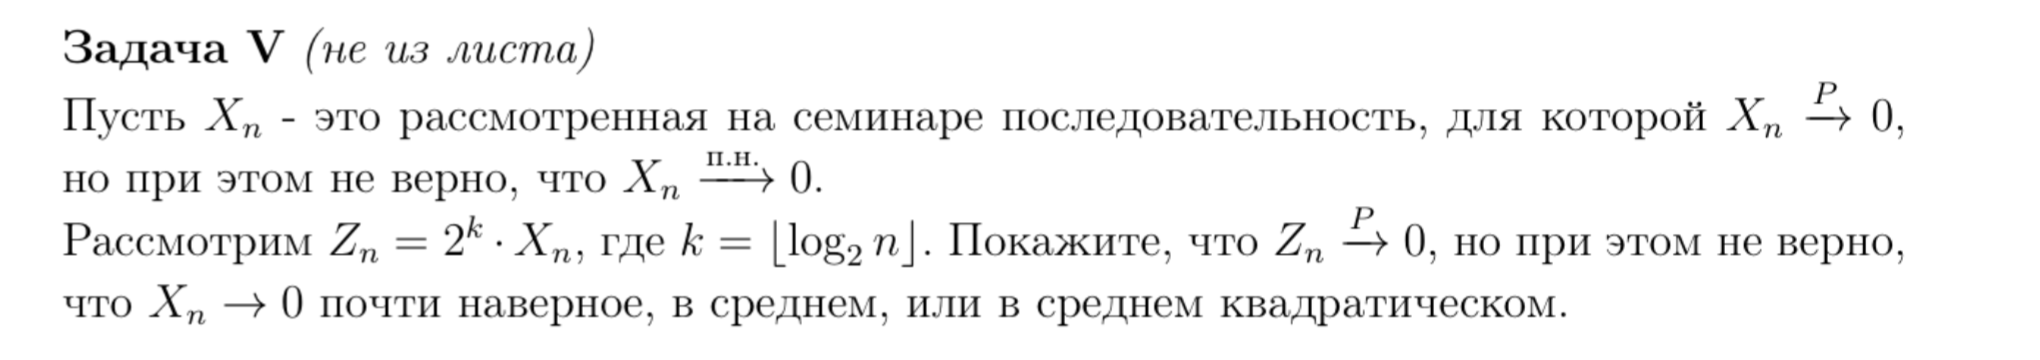
\includegraphics[scale=0.4]{4.png}
\end{center} 
Определяем $Z_n$, $X_n$ берем 1 в 1 с сема:
\[
 Z_n = 2^k \cdot X_n = 2^k \cdot
 I_{
\{
x \in  \left[
\frac{n - 2^k}{2^k}, \frac{n - 2^k + 1}{2^k}
\right]
\}
}
\]
На семе определили:

\begin{center}
\begin{tabular}{|c|c|c|}
\hline
 $X_n$& $0$ & $1$ \\
\hline
 $P$& $1 - \frac{1}{2^k}$ &  $\frac{1}{2^k}$\\
\hline
\end{tabular}
\end{center}
Аналогично для $Z_n$ будет:

\begin{center}
\begin{tabular}{|c|c|c|}
\hline
 $Z_n$& $0$ & $2^k$ \\
\hline
 $P$& $1 - \frac{1}{2^k}$ &  $\frac{1}{2^k}$\\
\hline
\end{tabular}
\end{center}
Теперь можем решать
\subsection*{1) $Z_n \overset{P}{\longrightarrow} 0$}
Проверяем:
\[
\forall \varepsilon > 0 : \lim_{n \rightarrow \infty} P \left(|Z_n| \geq \varepsilon \right) = 0?
\]
Смотрим:
\[
P (Z_n \geq \varepsilon) \leq P(Z_n \neq 0) = P(Z_n = 2^k) = \frac{1}{2^k}
\]
$k = [\log_2 n]$. В пределе получаем:
\[
\lim_{n \rightarrow \infty} P \left(|Z_n| \geq \varepsilon \right) = \lim_{n \rightarrow \infty} \frac{1}{2^{[\log_2 n]}} = \lim_{n \rightarrow \infty} \frac{1}{n} = 0 
\]
Стремление к нулю есть, значит есть сходимость по вероятности
\[
Z_n \overset{P}{\longrightarrow} 0
\]
\begin{center}
\textbf{Ч.Т.Д} 
\end{center}
\section*{2) $Z_n \overset{L_1}{\longrightarrow} 0$}
Проверяем:
\[
\mathbb{E} |Z_n|  \rightarrow 0 ?
\]
Считаем мат.ожидание:
\[
\mathbb{E} |Z_n|  = \mathbb{E} Z_n = 2^k \cdot \mathbb{E}  I_{
\{
x \in  \left[
\frac{n - 2^k}{2^k}, \frac{n - 2^k + 1}{2^k}
\right]
\}
} 
=
2^k \cdot \frac{1}{2^k} 
= 1 \nrightarrow 0
\]
К нулю не стремится, значит нет сходимости в среднем к нулю
\[
Z_n \overset{L_1}{\nrightarrow} 0
\]
\begin{center}
\textbf{Ч.Т.Д} 
\end{center}
\section*{3)  $Z_n \overset{L_2}{\longrightarrow} 0$}
Проверяем:
\[
\mathbb{E} |Z_n^2|  \rightarrow 0 ?
\]
Считаем мат.ожидание:
\[
\mathbb{E} |Z_n^2|  = \mathbb{E} Z_n^2 = 2^{2k} \cdot \mathbb{E}  I_{
\{
x \in  \left[
\frac{n - 2^k}{2^k}, \frac{n - 2^k + 1}{2^k}
\right]
\}
} 
=
2^{2k} \cdot \frac{1}{2^k} 
= 2^k \nrightarrow 0
\]
К нулю не стремится, значит нет сходимости в среднем квадратичном
\[
Z_n \overset{L_2}{\nrightarrow} 0
\]
\begin{center}
\textbf{Ч.Т.Д} 
\end{center}
\end{document}
